\chapter{ド・ジッター地平線と宇宙論的確率}

\lectureoverview{地平線は単なる因果的境界ではない。定常観測者にとってそれは熱系である。地平線から固有距離\(\rho\)の位置に保持された温度計は\(1/(2\pi\rho)\)程度の温度を示すが、重力赤方偏移により遠方で見られる放射ははるかに低温になる。このブラックホールの教訓をド・ジッター空間に持ち込み、固定された地平線半径\(H^{-1}\)を導出し、観測者の静的パッチ計量を書き下す。講義の後半では熱力学をその落ち着かない帰結まで追う。有限なド・ジッターエントロピー、ポアンカレ再帰、ボルツマン脳、永久インフレーション、そして測度問題である。最後の議論では、弦理論の厳密な超対称構造と、我々の世界を記述するかもしれない依然として未知の枠組みとを区別する。}

\section{地平線が熱いとはどういうことか}

本講義の前に、その夜の方向性を決める問いから始める。

\begin{classroomqa}
\audiencequestion{宇宙論的地平線にはブラックホールは存在しない。それにもかかわらず、どのような機構によってそれは熱くなりうるのか。\lecturetimestamp{00:00:17}}
\lecturerresponse{機構はブラックホール地平線の場合と同じである。有用な問いは操作的である。地平線近くに保持された温度計は何を記録するのか、そして地平線から遠く離れた観測者にはどのような放射が届くのか。}
\end{classroomqa}

最初の実験は局所的である。任意の滑らかな非極端地平線から固定された固有距離\(\rho\)の位置に温度計を保持する。地平線に十分近づくと、幾何学は普遍的なリンドラー形式を持ち、温度計は次を読み取る。
\begin{equation}
T_{\rm local}(\rho)\simeq \frac{1}{2\pi\rho}
\label{eq:l09-local-temperature}
\end{equation}
単位は\(\hbar=c=k_B=1\)とする。定数を復元すると次を得る。
\begin{equation}
k_B T_{\rm local}(\rho)\simeq \frac{\hbar c}{2\pi\rho}.
\end{equation}
\(\rho\to0\)における発散は、落下する観測者が通常の物質的な炉に遭遇することを意味しない。それは、地平線のすぐ外側にとどまり、したがってますます激しく加速しなければならない観測者によって割り当てられる温度である。

冒頭の会話はまた、混同されやすい三つの概念を区別する。エネルギー、温度、エントロピーである。

\begin{classroomqa}
\audiencequestion{光子をブラックホールに送り込んだ場合、依然として同じエントロピーを測定するのか、それともエネルギーだけが変化するのか。\lecturetimestamp{00:01:22}}
\lecturerresponse{光子が地平線の背後で到達不能になると、追加の情報が隠されたことになる。ここで用いられる単純化されたビットの言葉では、一つの光子は一つの追加ビットを隠し、それによってエントロピーを増加させうる。エネルギー、温度、エントロピーは関係しているが、互換ではない。}
\end{classroomqa}

\editorialnote{物理的なブラックホールに対して、エントロピー変化は熱力学的に\(dS=dE/T_H\)によって固定される。エネルギーによらずすべての光子について普遍的に1ビットであるわけではない。1ビットという記述は本講義の情報理論的理想化である。}

地平線近傍領域は高周波の量子揺らぎを絶えず放出し再吸収している。地平線は、定常観測者にとってそれらの揺らぎを熱的にする。しかしこれは直ちに一つの難問を提起する。もしその領域が任意に熱いなら、なぜ遠方の観測者は任意に高エネルギーの光子によって目をくらまされないのか。

\section{赤方偏移とホーキング温度}

通常の熱い壁は、我々がそこから遠く離れて立っていても、高周波放射の源であり続ける。地平線は、その放射が重力赤方偏移を経て登らなければならない点で異なる。光子の速さは\(c\)のままであり、減少するのはそのエネルギーである。
\begin{equation}
E=\hbar\omega,
\qquad
\omega_{\rm received}<\omega_{\rm emitted}.
\end{equation}
講義で用いられたチョークの比喩は、この点までは有用である。投げ上げられた石は上昇するにつれて減速するが、光子は光速を保ちながらその振動数とエネルギーが減少する。

シュヴァルツシルトブラックホールについて、無限遠の観測者が測定する温度は次である。
\begin{equation}
T_H=\frac{1}{8\pi M}
\label{eq:l09-hawking-natural}
\end{equation}
単位は\(G_N=\hbar=c=k_B=1\)とする。通常の単位では、
\begin{equation}
T_H=\frac{\hbar c^3}{8\pi G_N M k_B}.
\label{eq:l09-hawking-full}
\end{equation}

\begin{figure}[htbp]
\centering
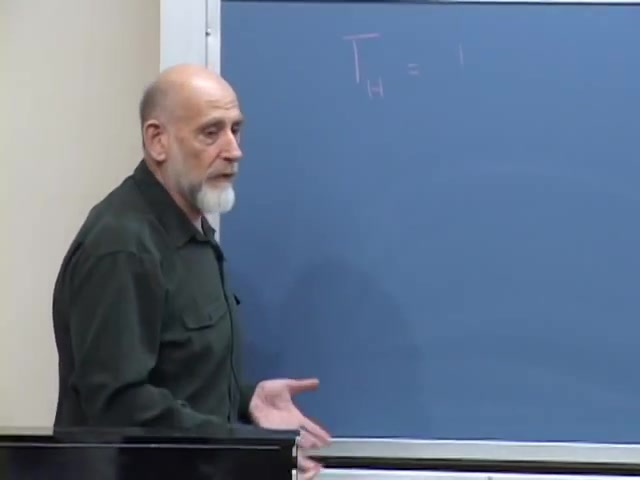
\includegraphics[width=0.68\textwidth]{lecture_09_figure_02.png}
\caption{自然単位でのホーキング温度\(T_H=1/(8\pi M)\)。}
\lectureframe{00:08:12}
\end{figure}

より大きなブラックホールはより低温である。講義ではこれを、典型的な光子を逆向きにたどることで説明する。熱的光子は特性エネルギー\(E_\gamma\sim T_H\)を持つ。\(M^{-1}\)程度のエネルギーで無限遠に到達する光子は、地平線近くを出発したときにはるかに大きな局所エネルギーを持っていた。地平線近傍の層と無限遠との間の赤方偏移は、より大きなブラックホールに対してより厳しくなり、より低い漸近温度を残す。

\begin{classroomqa}
\audiencequestion{もしシュヴァルツシルト時間が地平線で凍結するなら、もともと落下してブラックホールを形成した光子を追うべきではないのか。\lecturetimestamp{00:04:19}}
\lecturerresponse{温度の問題については、外向きに放出された光子を追えばよい。それらは非常に高い局所振動数で出発し、外へ登る間にエネルギーを失い、ホーキング放射として到達する。もともと落下した光子の運命は、別個の情報の問題である。}
\end{classroomqa}

\section{プランク層と引き伸ばされた地平線}

式~\eqref{eq:l09-local-temperature}の局所的な関係はどこまで信頼できるだろうか。この講義では、半古典的記述における意味を持つ最短距離としてプランク長を採用する。このことは、数学的な地平面のすぐ外側、およそプランク長一つ分の薄い層がプランクスケールの揺らぎで満たされていることを示唆する。それは絶えず放出と吸収を行っている。

放出された量子のほとんどは脱出しない。外向きの非常に狭い円錐へ向かうものだけが、落下して戻ることを免れる。一般的な角度で放たれた量子は地平面へ戻る。外向きと内向きの励起が衝突し、対やその他の粒子を生成する。この意味で、定常的な記述は極めて高温の物質の薄い殻を含んでいる。

\begin{figure}[htbp]
\centering
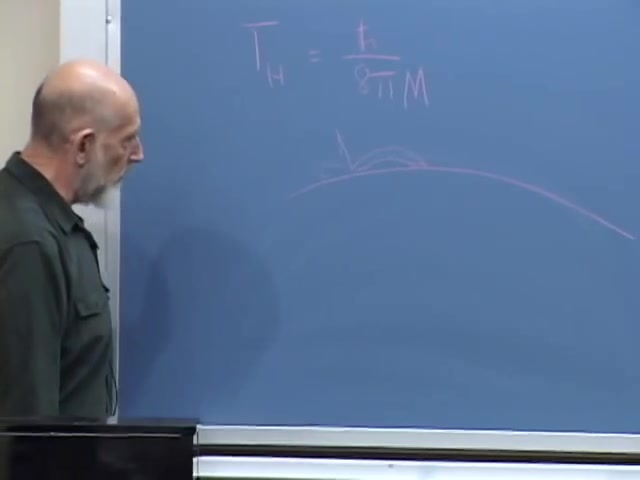
\includegraphics[width=0.74\textwidth]{lecture_09_figure_03.png}
\caption{地平面近傍の放射に対する狭い脱出円錐。局所的に放出された量子のほとんどは地平面へ戻る。}
\lectureframe{00:11:38}
\end{figure}

相補的な時空描像がある。地平面から離れては、仮想的な揺らぎは模式的に短い閉じたループで表されることがある。粒子・反粒子の励起が現れ、漸近状態になり得る前に消えるのである。地平面の近くでは、揺らぎは因果的境界をまたぐことができる。外部の観測者にとって、外側の部分は地平面から放出され、後に再吸収される粒子のように見える。ごくわずかな割合が脱出し、ホーキング放射となる。

\begin{classroomqa}
\audiencequestion{外部の図において、そのような揺らぎは\(t=-\infty\)から\(t=+\infty\)まで伸びるのか。\lecturetimestamp{00:15:00}}
\lecturerresponse{厳密な古典的地平面は、その特異に見える記述をもたらす。実際には、それを伸長地平面、すなわちおよそプランク長一つ分だけ外側にある時間的曲面で置き換える。すると放出と再吸収は有限の外部時間で起こる。}
\end{classroomqa}

\begin{figure}[htbp]
\centering
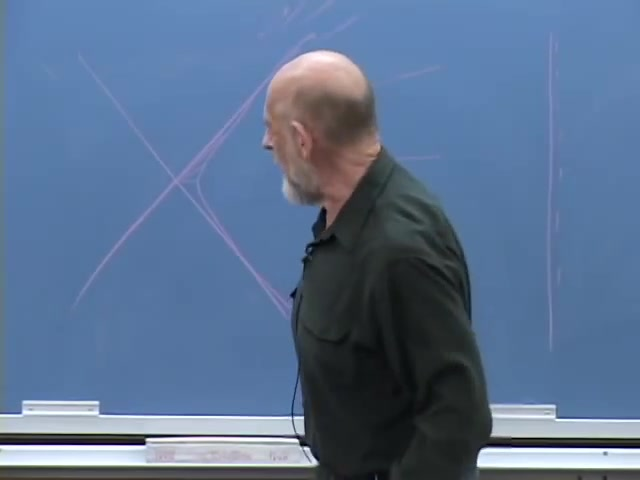
\includegraphics[width=0.72\textwidth]{lecture_09_figure_04.png}
\caption{古典的地平面と、外部記述で用いられる近傍の伸長地平面。}
\lectureframe{00:15:52}
\end{figure}

伸長地平面は新しい不変な境界ではない。それは半古典的幾何学が信頼できなくなる場所に置かれた有効な曲面である。物質および幾何学自体の量子揺らぎが、厳密な位置をプランクスケールでぼかす。この構成は、その不確定性を、外部記述が有限に保たれる曲面上にまとめ上げる。

この局所的な議論のどこにも、地平面がブラックホールに属するのか、加速する宇宙に属するのかを知る手がかりはない。それがド・ジッター空間への橋渡しである。

\section{膨張座標におけるド・ジッター空間}

正式な講義は、ド・ジッター時空の空間的に平坦なスライスから始まる。
\begin{equation}
ds^2=-dt^2+e^{2Ht}d\mathbf{x}^2,
\qquad
d\mathbf{x}^2=dx^2+dy^2+dz^2.
\label{eq:l09-flat-slicing}
\end{equation}
定数\(H\)はド・ジッター膨張率である。この因子が\(e^{2Ht}\)として現れるのは、計量が距離の二乗を測るからである。固定された座標間隔は物理的長さ
\begin{equation}
D(t)=e^{Ht}\lvert\Delta\mathbf{x}\rvert.
\end{equation}
を持つ。

\begin{figure}[htbp]
\centering
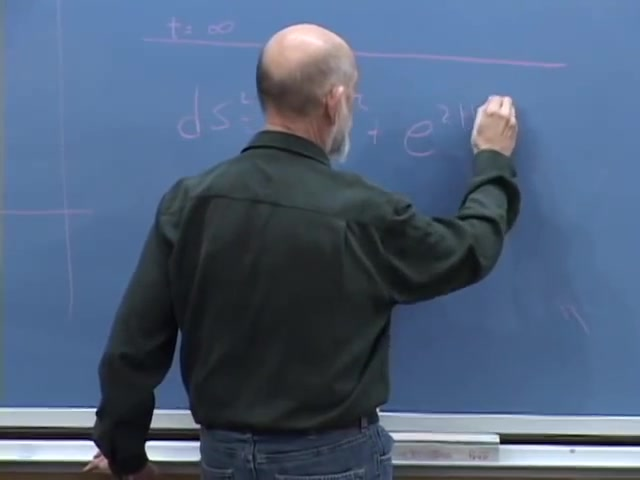
\includegraphics[width=0.78\textwidth]{lecture_09_figure_05.png}
\caption{平坦座標における指数的に膨張するド・ジッター計量。}
\lectureframe{00:18:50}
\end{figure}

これらの座標は膨張を明瞭にするが、未来の無限遠をページのはるか上方に置く。それを黒板に持ち込むために、共形時間を導入する。
\begin{equation}
\eta=-\frac{1}{H}e^{-Ht},
\qquad
-\infty<\eta<0.
\label{eq:l09-conformal-time}
\end{equation}
すると
\begin{equation}
dt=\frac{d\eta}{-H\eta},
\qquad
e^{Ht}=-\frac{1}{H\eta},
\end{equation}
であり、式~\eqref{eq:l09-flat-slicing}は
\begin{equation}
ds^2=\frac{1}{H^2\eta^2}
\left(-d\eta^2+d\mathbf{x}^2\right).
\label{eq:l09-conformal-metric}
\end{equation}
となる。\(t\to+\infty\)のとき、\(\eta\to0^{-}\)である。無限の固有時間が、有限の水平線\(\eta=0\)へ圧縮されたのである。

\editorialnote{時間の変換は黒板に書いている間に何度か修正される。式~\eqref{eq:l09-conformal-time}が整合的な形である。初期の宇宙時間は\(\eta\to-\infty\)へ写り、未来の無限遠は\(\eta\to0^{-}\)へ写る。}

\begin{figure}[htbp]
\centering
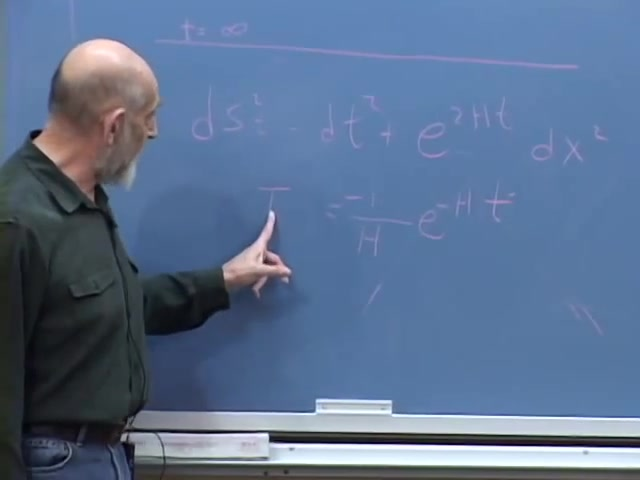
\includegraphics[width=0.82\textwidth]{lecture_09_figure_06.png}
\caption{共形時間の変換と共形的に平坦な計量。}
\lectureframe{00:21:24}
\end{figure}

共形因子は時間項と空間項の両方に掛かるので、ヌル方向を変えない。動径方向の光線に対して
\begin{equation}
ds^2=0
\quad\Longrightarrow\quad
-d\eta^2+dx^2=0
\quad\Longrightarrow\quad
\frac{dx}{d\eta}=\pm1.
\label{eq:l09-null-rays}
\end{equation}
したがって光は共形図において\(45^\circ\)で進む。これが座標変換が有用である理由である。因果的可到達性が見えるようになるのである。

\section{一人の観測者の因果的パッチ}

世界線が無限の固有時間にわたって続く観測者を想像しよう。コンパクト化された図では、それは\(\eta=0\)上の一点で終わる。その観測者が受け取ることのできるあらゆる信号は、その端点の過去光円錐の内側にある。円錐の外側の事象は、観測者がどれほど長く待っても、その観測者と決して通信できない。

\begin{figure}[htbp]
\centering
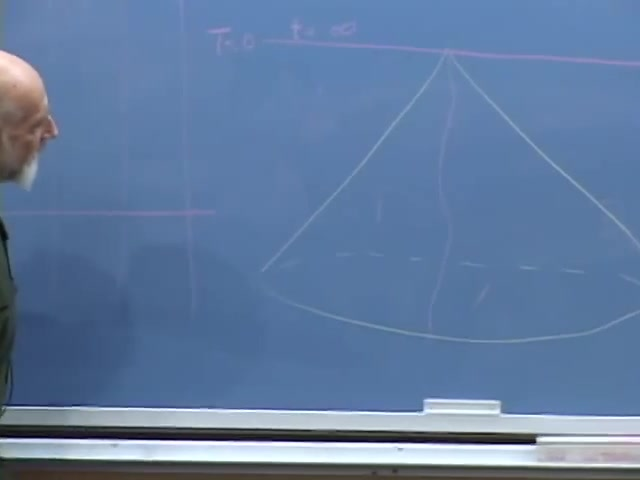
\includegraphics[width=0.78\textwidth]{lecture_09_figure_07.png}
\caption{共形ド・ジッター座標における観測者の極限的な過去光円錐。}
\lectureframe{00:24:38}
\end{figure}

第二の観測者は異なる円錐を持つ。二つの可到達領域は重なるが、どちらも時空全体ではない。以下の議論では第一の観測者の視点を採用し、その過去光円錐をその観測者の因果的パッチと呼ぶ。

図はパッチが未来に向かって縮むように見えるが、座標幅は固有距離ではない。一定の\(\eta\)スライス上で、\(x=0\)にいる観測者と\(x=\Delta x\)にある地平線との間の物理的距離の二乗は
\begin{equation}
D^2=\frac{(\Delta x)^2}{H^2\eta^2}.
\label{eq:l09-horizon-distance-start}
\end{equation}
である。地平線は\(\eta=0\)で終わる\(45^\circ\)のヌル線であるから、
\begin{equation}
\Delta x=\lvert\eta\rvert.
\end{equation}
となる。代入すると
\begin{equation}
D_{\rm hor}^2=\frac{1}{H^2},
\qquad
D_{\rm hor}=\frac{1}{H}.
\label{eq:l09-horizon-radius}
\end{equation}
が得られる。座標間隔は縮むが、共形因子はちょうど補償する分だけ大きくなる。固有地平線半径は一定である。

\begin{figure}[htbp]
\centering
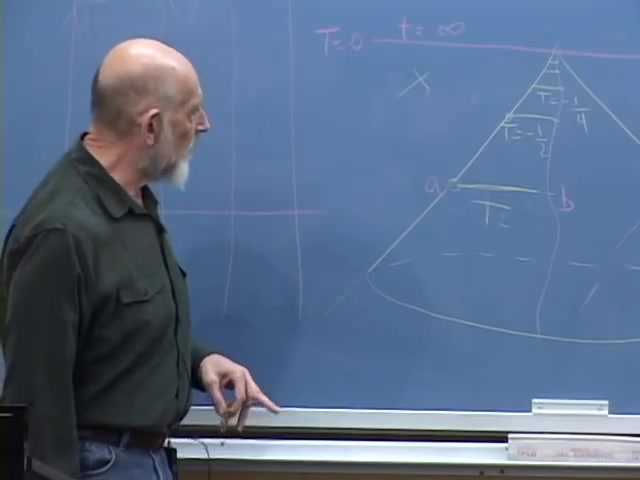
\includegraphics[width=0.80\textwidth]{lecture_09_figure_08.png}
\caption{縮む座標間隔を固定された固有距離\(H^{-1}\)に変換する板書の導出。}
\lectureframe{00:28:42}
\end{figure}

\section{静的パッチ}

地平線半径が固定されていることは、中心の観測者に適合した座標を示唆する。座標変換を導出することなく、講義は結果を次のように書く：
\begin{equation}
ds^2=
-\left(1-H^2r^2\right)d\tau^2
+\frac{dr^2}{1-H^2r^2}
+r^2d\Omega_2^2.
\label{eq:l09-static-patch}
\end{equation}
係数は\(\tau\)ではなく\(r\)に依存する。このチャートは観測者の静的パッチを覆い、
\begin{equation}
0\le r<\frac{1}{H}.
\end{equation}

\begin{figure}[htbp]
\centering
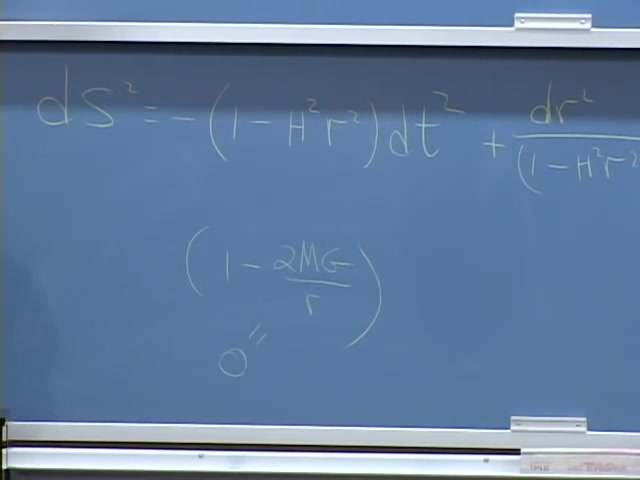
\includegraphics[width=0.88\textwidth]{lecture_09_figure_09.png}
\caption{ド・ジッター静的パッチ計量と、シュヴァルツシルト因子との比較。}
\lectureframe{00:34:22}
\end{figure}

シュヴァルツシルトとの類似は即座に明らかである：
\begin{equation}
f_{\rm dS}(r)=1-H^2r^2,
\qquad
f_{\rm Schw}(r)=1-\frac{2G_NM}{r}.
\end{equation}
いずれの場合も、静的座標の地平線は\(f(r)=0\)となる場所に現れる。ド・ジッターの場合、
\begin{equation}
1-H^2r^2=0
\quad\Longrightarrow\quad
r_H=H^{-1}.
\end{equation}
このチャートはそこで特異であり、ちょうどシュヴァルツシルト座標がブラックホールの地平線で特異であるのと同じである。それにもかかわらず、大域的な幾何学は重要な点で異なる。ブラックホールの観測者は外側に立って内側を見る。ド・ジッターの観測者は内側に立って外側を見る。

\begin{classroomqa}
\audiencequestion{自由に放たれた粒子が指数関数的に膨張する宇宙で互いに離れていくとき、幾何学が静的でありうるのはなぜか。\lecturetimestamp{00:36:06}}
\lecturerresponse{静的とは、すべての粒子が固定されているという意味ではない。計量の係数と、繰り返された実験の結果が開始時刻に依存しないという意味である。今、二つの粒子を放てばそれらは加速しながら離れていく。同じ実験を後で繰り返せば、同じ運動が起こる。}
\end{classroomqa}

\begin{classroomqa}
\audiencequestion{離れていく二つの粒子は互いに赤方偏移を見るか。\lecturetimestamp{00:38:34}}
\lecturerresponse{はい。観測者に適合した計量が時間に依存しなくても、それらの間隔が増大することは相対的な赤方偏移を生む。}
\end{classroomqa}

\section{内側から見た温度}

シュヴァルツシルト空間とド・ジッター空間の地平線近傍の構造は局所的に等価である。したがってド・ジッター地平線は熱的量子を放出し再吸収する。まれな光子は中心の観測者へ内向きに伝播し、静的パッチのポテンシャルを登るにつれてエネルギーを失う。中心で測定されるギボンズ--ホーキング温度は
\begin{equation}
T_{\rm dS}=\frac{H}{2\pi}
\label{eq:l09-de-sitter-temperature}
\end{equation}
であり、自然単位を用いている。半径\(r\)にある静止した温度計はトールマン赤方偏移された値
\begin{equation}
T_{\rm local}(r)=
\frac{T_{\rm dS}}{\sqrt{1-H^2r^2}},
\label{eq:l09-tolman}
\end{equation}
を読み取り、これは\(r\to H^{-1}\)として発散し、地平線近くでは式~\eqref{eq:l09-local-temperature}に帰着する。

\editorialnote{講義は式~\eqref{eq:l09-de-sitter-temperature}と\eqref{eq:l09-tolman}を明示的に書く代わりに、地平線距離と赤方偏移からスケールを導出する。それらはその議論の標準的な規格化を述べている。}

観測された晩期の加速に対して、講義は期間の推定値
\begin{equation}
H^{-1}\sim 20\times10^9\ {\rm light\ years}.
\label{eq:l09-lecture-horizon-estimate}
\end{equation}
を用いる。すると典型的な地平線光子は数十億光年に匹敵する波長を持つ。これはマイクロ波背景放射ではない。はるかに低温である。

操作的思考実験は宇宙論的スケールの釣り竿である。アリスは\(r=0\)にとどまり、データも伝送する非常に長い糸に温度計を取り付け、宇宙の斥力に計器を外側へ運ばせる。彼女はそれを地平線のすぐ手前で止め、信号が戻るのを待つと、大きな局所温度を見出す。中心で彼女のそばにある温度計は微小な値\(H/(2\pi)\)を読み取る。一つの地平線が両方の読みを支えるのは、それらが異なる重力ポテンシャルで行われるからである。

\section{地平線の横断}

古典的な外側の記述は、よく知られたブラックホールの話に似ている。中心にいるボブはアリスが遠ざかるのを見る。彼女の信号はますます赤方偏移し、ますますゆっくりと到着する。彼女は地平線に押しつぶされて見え、最終的に薄れていく。後から来る旅行者ジェーンは、境界近くの堆積層の中のもう一つのより薄い層として現れる。

\begin{classroomqa}
\audiencequestion{我々の視点から、物体はかつて宇宙の地平線を通り抜けるのか。\lecturetimestamp{00:45:30}}
\lecturerresponse{静的観測者の古典的記述では通り抜けない。それらの信号は赤方偏移して薄れ、見かけの位置は地平線に近づく。しかし、それら自身の自由落下の記述では、それらは局所的に特異な面に出会うことなく横断する。}
\end{classroomqa}

\begin{classroomqa}
\audiencequestion{地平線が熱いのは、そこを越えずに近くにとどまる観測者にとってだけなのだろうか？落下する観測者は、ただ通過するだけで焼かれてしまうわけではないのだろう？\lecturetimestamp{00:48:27}}
\lecturerresponse{アリスは自身の座標系では滑らかに越えていく。極端な温度は静止した記述に属する。ボブがアリスを地平線にどこまでも近づけて分解しようと固執するなら、彼はますます短い波長でアリスを照らさなければならない。その試みられたハイゼンベルク顕微鏡は、観測しようとするものを焼くのに十分なエネルギーを注ぎ込むことになる。}
\end{classroomqa}

これは二つの局所的な事象の間の矛盾ではない。静止した観測者と落下する観測者は根本的に異なる測定を用いている。地平線相補性は、一方の観測者が重複した情報を直接比較することを許さずに、どのようにして両方の記述が妥当でありうるかを問うものである。

\section{真空の斥力のニュートン模型}

この時点で、学生がブラックホールの重力井戸に代わるものは何かと尋ねる。サスキンドはニュートン模型を構成することで答える。\(\phi\) を重力ポテンシャルとすると、試験粒子の加速度は
\begin{equation}
\mathbf{a}=-\boldsymbol{\nabla}\phi.
\end{equation}
通常の非相対論的物質に対しては、ポアソン方程式は
\begin{equation}
\nabla^2\phi=4\pi G_N\rho.
\label{eq:l09-poisson}
\end{equation}

\begin{classroomqa}
\audiencequestion{ブラックホールの効果がその重力井戸から来るのなら、ド・ジッター空間における対応する源は何か？\lecturetimestamp{00:49:36}}
\lecturerresponse{真空エネルギー自体が空間的に一様な重力源を与える。ニュートン的記述では、それは \(1/r\) の井戸ではなく二次のポテンシャルを生じる。}
\end{classroomqa}

\begin{figure}[htbp]
\centering
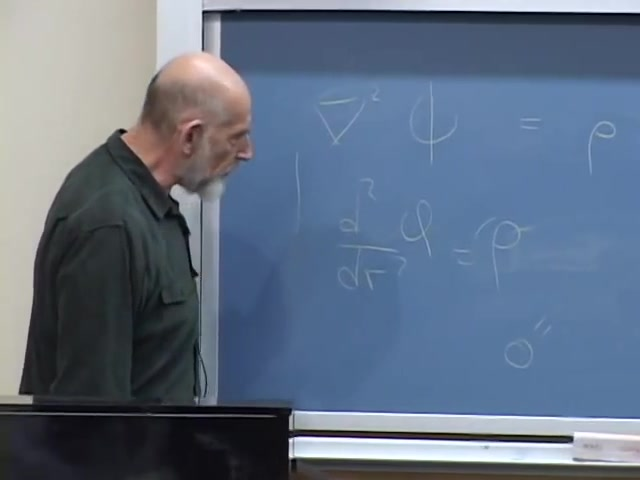
\includegraphics[width=0.78\textwidth]{lecture_09_figure_10.png}
\caption{ポアソン方程式と、講義で用いられた模式的な動径方向二階微分の形。}
\lectureframe{00:51:38}
\end{figure}

板書では規格化、球面測度の項、圧力、そして当初は全体の符号さえも省かれ、演習は
\begin{equation}
\frac{d^2\phi}{dr^2}\sim H^2.
\end{equation}
に還元される。本質的な推論は、一定の源が二次関数を与えるということである。ド・ジッター斥力に必要な符号をとると、
\begin{equation}
\phi_{\rm dS}(r)=-\frac{1}{2}H^2r^2,
\qquad
a_r=-\frac{d\phi_{\rm dS}}{dr}=H^2r.
\label{eq:l09-de-sitter-potential}
\end{equation}
加速度は外向きを向き、距離に比例して増大する。\(\ddot r=H^2r\) を解くと
\begin{equation}
r(\tau)=A e^{H\tau}+B e^{-H\tau},
\end{equation}
となり、増大する枝が指数的な分離を再現する。

\begin{figure}[htbp]
\centering
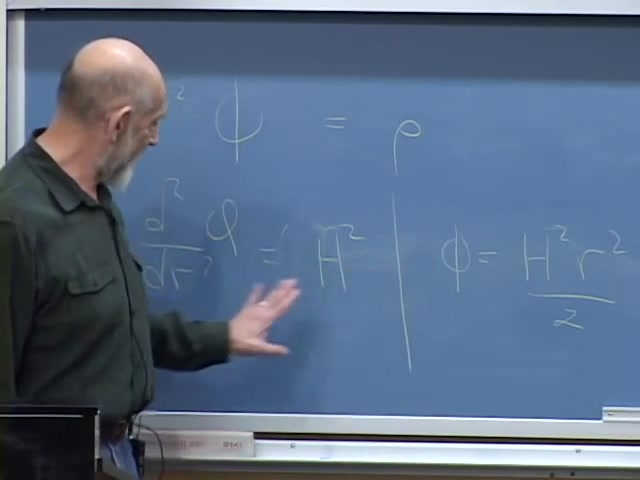
\includegraphics[width=0.76\textwidth]{lecture_09_figure_11.png}
\caption{一様な源の方程式と、二次のド・ジッターポテンシャル。}
\lectureframe{00:53:32}
\end{figure}

\editorialnote{一般相対論では、一様な流体の弱場加速度は \(\rho+3p\) に依存し、\(\rho\) だけには依存しない。真空エネルギーは \(p=-\rho\) をもつので、\(\rho+3p=-2\rho\) となり、加速度は斥力的である。式~\eqref{eq:l09-de-sitter-potential} は正しく規格化されたド・ジッターの結果であり、板書の計算は意図的に二次の依存性と符号のみを追っている。}

中心に通常の質量 \(M\) を置く。定性的なポテンシャルは
\begin{equation}
\phi(r)=-\frac{G_NM}{r}-\frac{1}{2}H^2r^2,
\label{eq:l09-combined-potential}
\end{equation}
となり、動径方向の加速度は
\begin{equation}
a_r=-\frac{G_NM}{r^2}+H^2r.
\end{equation}
である。小さい \(r\) では局所的な引力が勝ち、大きい \(r\) では真空の斥力が勝つ。それらの釣り合いは
\begin{equation}
r_\ast=\left(\frac{G_NM}{H^2}\right)^{1/3}.
\label{eq:l09-turnaround}
\end{equation}
で起こる。これは講義におけるポテンシャルの極大のきれいな版である。近くの重力束縛系がまとまったままでいられる一方、十分に遠い銀河が加速して遠ざかる理由を定性的に説明する。

\begin{figure}[htbp]
\centering
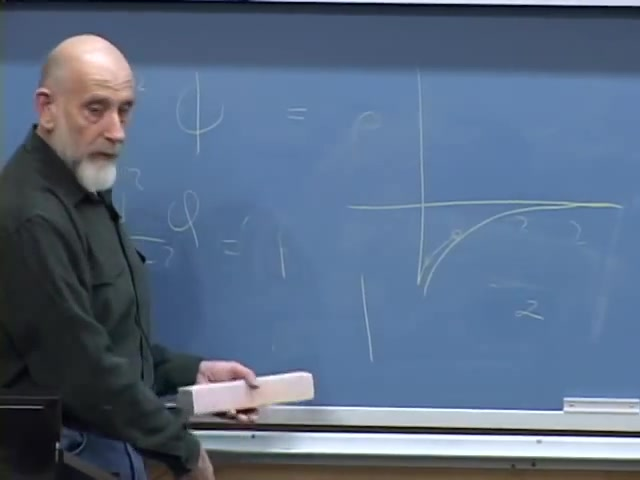
\includegraphics[width=0.78\textwidth]{lecture_09_figure_12.png}
\caption{通常の \(1/r\) 引力と、逆さまの二次のド・ジッターポテンシャルとの組み合わせ。}
\lectureframe{00:58:20}
\end{figure}

\begin{classroomqa}
\audiencequestion{通常の力は依然として重要か、それとも真空の斥力が最終的にあらゆる物質の島を引き裂くのか？\lecturetimestamp{00:57:29}}
\lecturerresponse{すべての力を含めなければならない。十分に小さいスケールでは、電磁気的な束縛と局所的な重力が支配する。真空の斥力が重要になるのは、\(H^{-1}\) と、束縛された質量に応じた釣り合いのスケールによって定まる巨大な距離を越えてのみである。}
\end{classroomqa}

\section{一つの源、いくつかの名前}

ここで議論は用語をめぐって小休止する。真空エネルギー、宇宙定数、暗黒エネルギーは、用いられている模型における三つの加算的な実体ではない。それらは同じ \(w=-1\) の源についての三つの記述である。アインシュタイン方程式における定数項、真空のローレンツ不変なエネルギー密度、あるいは後期の加速を駆動する成分について語ることができる。

\begin{classroomqa}
\audiencequestion{一様なニュートン的源と量子真空エネルギーは、別々の効果として両方存在するのか？\lecturetimestamp{00:59:14}}
\lecturerresponse{いいえ。一様な密度は同じ源のニュートン模型である。真空エネルギー、宇宙定数、そしてこの講義では暗黒エネルギーは、一つの物理的成分を指す。}
\end{classroomqa}

\begin{classroomqa}
\audiencequestion{それでは、同じ現象が古典的な記述と量子的な記述の両方をもつことになるのでしょうか。\lecturetimestamp{01:00:32}}
\lecturerresponse{その微視的起源は量子力学的でありうる。ちょうど電子の質量の一部が量子的起源をもつように。有効エネルギー密度がわかれば、それは通常の源として古典的な重力方程式に入る。観測された値の究極の起源はわかっていない。}
\end{classroomqa}

プランク単位では、観測されている真空エネルギー密度は極めて小さく、
\begin{equation}
\rho_\Lambda\sim10^{-123}\rho_{\rm Pl},
\label{eq:l09-planck-smallness}
\end{equation}
プランク密度に用いる規約にもよるが、その程度である。この小さな数が宇宙定数問題である。また、それゆえに地平線がこれほど大きいのである。4次元では、
\begin{equation}
H^2=\frac{8\pi G_N}{3}\rho_\Lambda,
\qquad
r_H=H^{-1}.
\end{equation}
もし\(H\)がより大きければ、地平線はより小さくなり、中心のド・ジッター温度はより高くなり、斥力的加速度\(H^2r\)はより強くなるであろう。

\begin{classroomqa}
\audiencequestion{この微小な宇宙定数は、プランク定数や量子ゆらぎと関係しているのでしょうか。\lecturetimestamp{01:03:27}}
\lecturerresponse{きれいな比較には無次元のプランク単位が用いられ、そこでは\(G_N=\hbar=c=1\)である。その単位では、真空密度は自然なプランク密度よりおよそ\(123\)桁小さい。この階層性を説明することは、基礎物理学の中心的難問の一つである。}
\end{classroomqa}

\begin{classroomqa}
\audiencequestion{真空エネルギーは厳密に一定の宇宙定数でなければならないのでしょうか。加速成分が減少し、最終的にゼロに落ち着くことはありえませんか。\lecturetimestamp{01:04:52}}
\lecturerresponse{それは論理的に可能な代替案である。すなわち、動的な暗黒エネルギー場が時間とともに変化しうる。講義では一定の場合を採用している。それは、当時利用可能な観測が宇宙定数に近い振る舞いをますます支持していたからであり、あらゆる代替案が不可能であると証明されていたからではない。}
\end{classroomqa}

\section{遠い未来の天文学}

漸近的にド・ジッター的な宇宙では、重力で束縛されていない構造はやがて観測者の地平線を越える。宇宙マイクロ波背景放射は検出限界以下に赤方偏移する。遠方の銀河は消える。生き残った天文学者は、そうでなければ暗い領域の中に、合体した局所的な重力の島だけを見るかもしれない。

\begin{classroomqa}
\audiencequestion{望遠鏡がなければ、遠方の銀河が消えたことに誰か気づくことさえあるでしょうか。\lecturetimestamp{01:06:17}}
\lecturerresponse{おそらくないであろう。深刻な問題はもっと深い。高度な観測機器があっても、未来の観測者は、今日われわれが膨張を推測するもととなる遠方のトレーサーやマイクロ波背景放射を欠くかもしれない。}
\end{classroomqa}

そのとき、古い島宇宙像が説得力をもつように見えるかもしれない。オルバースのパラドックスは別の結論を強いることはないであろう。なぜならそれは、無限で静的で一様な発光源の集団を仮定しているからであり、未来の観測者は局所的な島の有限個の恒星だけを見るであろう。暗黒エネルギーが空虚な空間から絶えず代わりの銀河を作り出すわけではない。

厳密なド・ジッター空間における地平線は、局所的な銀河の周りで縮まない。その物理的半径は\(H^{-1}\)のままであり、銀河よりはるかに大きい。消えるのは、その固定された因果的境界の向こうへ運ばれた束縛されていない物質である。

\begin{classroomqa}
\audiencequestion{銀河から放出された恒星は、大規模な幾何学を検出するための試験体として役立ちうるでしょうか。\lecturetimestamp{01:11:25}}
\lecturerresponse{しばらくの間は、役立つ。放出された天体や長基線の光信号は幾何学を探ることができる。しかし、その効果が有意になるのは10億光年の相当な割合程度の距離にわたってのみであり、したがってその実験には宇宙論的な時間がかかるであろう。}
\end{classroomqa}

\begin{classroomqa}
\audiencequestion{遠方の地平線がすでに宇宙の大部分をわれわれから隠しているのではないと、どうしてわかるのでしょうか。\lecturetimestamp{01:11:45}}
\lecturerresponse{われわれはすでに十分な数の銀河、赤方偏移、背景放射を見ており、膨張を測定し、大規模な幾何学を再構成できる。それらのトレーサーを奪われた未来の観測者は、はるかに難しい推論の問題に直面するであろう。}
\end{classroomqa}

\begin{classroomqa}
\audiencequestion{もし地平線がアンドロメダのすぐ向こうにあるなら、その存在は明らかでしょうか。\lecturetimestamp{01:12:19}}
\lecturerresponse{はい。そのように小さな地平線は、はるかに大きな\(H\)を必要とし、その結果生じる斥力はアンドロメダの運動を強く変えるであろう。測定された値はむしろ、漸近的な地平線をはるかに大きなスケールに置く。}
\end{classroomqa}

\begin{classroomqa}
\audiencequestion{われわれの地平線の向こうで新しいビッグバンが起こっていることはありえませんか。\lecturetimestamp{01:13:25}}
\lecturerresponse{地平線の向こうの事象は、われわれにもわれわれの子孫にも見えない。関連するがより精密な可能性である、永遠のインフレーションにおける泡の核生成については、講義の後半で導入する。}
\end{classroomqa}

ロケットと時計、そして数十億年があれば、未来の観測者は探検者たちをパッチの大部分にわたって送り込み、その計量を再構成できるだろう。しかし通常の実験室規模や文明規模の時間スケールでは、この効果はほとんど到達不可能である。この区別は、膨張を発見することは不可能であろうという過度に強い主張を正す。それは操作上はるかに遠いのであって、原理的に禁じられているのではない。

\begin{classroomqa}
\audiencequestion{未来の探検者たちは、熱的再帰を待つよりもずっと早く幾何を決定できるだろうか。\lecturetimestamp{01:21:40}}
\lecturerresponse{もちろんである。再帰は提案された測定ではない。数十億光年の基線にわたって光信号を交換する探検者たちは、はるかに短い、しかしそれでも宇宙論的な時間スケールで静的パッチを地図化できるだろう。}
\end{classroomqa}

\begin{classroomqa}
\audiencequestion{赤方偏移は、そのような探検者たちが返すすべての情報を消し去ってしまうだろうか。\lecturetimestamp{01:23:24}}
\lecturerresponse{彼らが地平線のはるか内側のスケールを探るのであれば、そうはならない。数十億光年程度の基線は、中程度の赤方偏移しか生じないにもかかわらず、すでに膨張に敏感である。この実験は主としてその膨大な持続時間によって制限される。}
\end{classroomqa}

\section{有限エントロピーと再帰}

静的パッチは熱力学的な意味で空ではない。その地平線は面積
\begin{equation}
A_H=4\pi H^{-2},
\end{equation}
温度\(T_{\rm dS}=H/(2\pi)\)、そしてエントロピー
\begin{equation}
S_{\rm dS}=\frac{A_H}{4G_N}
=\frac{\pi}{G_NH^2}
\label{eq:l09-de-sitter-entropy}
\end{equation}
を持ち、単位は\(\hbar=c=k_B=1\)である。エントロピーは有限である。したがって、静的パッチを、適切な注意を払いつつ、定常的な記述において励起が地平線近くに集中する有限エントロピーの熱的キャビティとして思い描いてもよい。

平衡状態にある通常の気体の箱は、短い時間スケールでは特徴のないものに見えるが、統計力学は揺らぎを禁じてはいない。あるマクロ状態が平衡状態に対してエントロピー不足\(\Delta S\)を持つならば、その確率はおよそ
\begin{equation}
P\sim e^{-\Delta S}.
\label{eq:l09-fluctuation-probability}
\end{equation}
である。対応する待ち時間は
\begin{equation}
t\sim t_0 e^{\Delta S}.
\end{equation}
のように増大する。有限な系では、それ以前の状態に任意に近い状態を再訪するまでの時間はポアンカレ再帰時間であり、
\begin{equation}
t_{\rm rec}\sim H^{-1}e^{S_{\rm dS}}.
\label{eq:l09-recurrence}
\end{equation}
である。我々の地平線に対する\(S_{\rm dS}\)は\(10^{120}\)の程度であるから、講義ではそのスケールを\(e^{10^{120}}\)と要約する。前因子が年で測られようと、ハッブル時間で測られようと、微視的な単位で測られようと、二重指数の前では無関係である。

\begin{figure}[htbp]
\centering
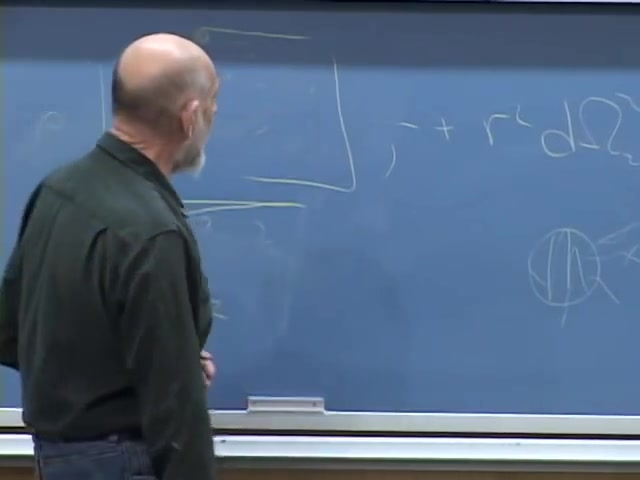
\includegraphics[width=0.76\textwidth]{lecture_09_figure_13.png}
\caption{黒板に書かれた、膨大な指数関数的待ち時間スケールを伴う再帰の議論。}
\lectureframe{01:16:24}
\end{figure}

そのような再帰の前には、より小さな揺らぎのほうがはるかに頻繁に起こる。部屋の中の分子がすべて一隅に集まることもあるかもしれない。複雑な渦が一時的に形成されることもあるかもしれない。講義の遊び心ある階層では、熱運動が象を組み立てることもあるかもしれない。要求されるエントロピー不足が小さいほど、その揺らぎはより安価である。

\begin{classroomqa}
\audiencequestion{ポアンカレ再帰は特に量子力学の帰結なのか。\lecturetimestamp{01:25:44}}
\lecturerresponse{いいえ。再帰と稀な揺らぎはすでに古典統計力学において生じる。それらをド・ジッター空間に適用する際には我々の現在の物理的枠組みを用いるが、それはいつか改訂されるかもしれない。しかし熱力学と統計的推論は、我々が知る最も頑健な構造の一つである。}
\end{classroomqa}

確率そのものの意味は、将来の理論においてより深まるかもしれない。サスキンドはそうでないとは主張していない。彼のより狭い論点は、統計力学の長期的な含意が奇妙であるというだけの理由でそれを放棄することは、物理学で最もよく検証された組織原理の一つを捨て去ることになる、というものである。

\section{ボルツマン脳と典型的観測者}

熱的な揺らぎがビッグバンのような状態全体を創り出すと仮定しよう。それには膨大なエントロピー減少が必要である。一つの太陽系を生み出す揺らぎはより安価であり、すでに暖かい地球はさらに安価である。唯一の要件が一人の観測者であるならば、最も費用のかからない揺らぎは、見かけの記憶を備えた機能する脳だけを創り出すかもしれない。そのような仮説的観測者はボルツマン脳と呼ばれる。

問題は、一つの奇妙な揺らぎが論理的に可能かどうかではない。ある宇宙論的モデルが、ほとんどすべての観測者はそのような揺らぎであると予測するかどうかである。我々は、自分たちが途方もなく非典型的であるとは仮定しないことによって、観測から推論する。首尾一貫した宇宙史を持つ通常の観測者が、孤立した熱的脳によって指数関数的に圧倒される理論は、その推論を損なう。

したがってボルツマン脳問題は、定量的な整合性のテストを名指ししている。通常の観測者の期待される存在量と、揺らぎから生まれた観測者の存在量を比較する。後者が支配するならば、それらが増殖する前に真空が崩壊しなければならないか、測度を変更しなければならないか、あるいは宇宙論的仮定を再検討しなければならない。

紫外--赤外の繋がりに関する以前の問いは、明示的に先送りされる。再帰の議論は、その別個の問題を解決することに依存していない。

\section{永遠のインフレーションと泡宇宙}

次に講義は、完全な導出を試みることなく、第二の確率問題を導入する。準安定なド・ジッター真空は、真空エネルギーがより低い泡を核生成しうる。泡の壁は膨張し、その内部は開いたフリードマン--ロバートソン--ウォーカー宇宙へと発展しうる。一方、周囲のインフレーション領域は膨張を続け、さらに多くの泡を核生成する。

\begin{figure}[htbp]
\centering
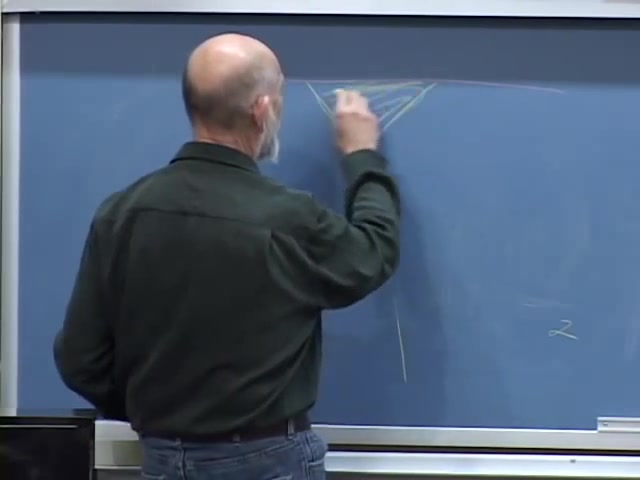
\includegraphics[width=0.74\textwidth]{lecture_09_figure_14.png}
\caption{膨張するド・ジッター背景の内部に描かれた、より低い真空エネルギーの泡。}
\lectureframe{01:29:38}
\end{figure}

決定的な特徴は指数関数的な個体数の増加である。新しい物理的体積は泡がそれを取り除くよりも速く生成されるため、泡領域の数は際限なく増大する。異なる泡は異なる低エネルギー状態に落ち着き、したがって異なる有効物理を示しうる。

統計的な困難を明らかにするため、サスキンドはまず宇宙論を離れ、有限だが未知の資源を持つ指数関数的に増加する人類人口を考える。観測者はこれまでに生きるすべての人々の中で典型的であると仮定する。人口が各世代で倍増し、その後終わるとすれば、全人類の半分は最後の世代に生き、四分の三は最後の二世代に生き、八分の七は最後の三世代に生きる：
\begin{equation}
f_n=1-2^{-n}.
\label{eq:l09-last-generations}
\end{equation}
その場合、典型性は、全資源供給について何も知らないにもかかわらず、われわれを不快なほど終末の近くに位置づける。これは人類絶滅の信頼できる予測として提示されているのではない。指数関数的成長が、数の集計をカットオフに支配させるという警告である。

コイン投げの例は、通常の典型性仮定をより明快に述べている。多数の実験者がそれぞれ公正なコインを\(N\)回投げるなら、圧倒的多数は
\begin{equation}
n_H=\frac{N}{2}+O(\sqrt{N}).
\end{equation}
を得る。極端な観測者は、証拠なしに自分が途方もなく稀な裾に位置すると仮定するよりも、まず悪いモデルか悪いコインを疑うべきである。宇宙論的確率も同じ典型性の直観を用いるが、無限の母集団においては、数を数えるための明確に定義された方法を必要とする。

\section{エッシャーの境界と測度問題}

サスキンドの幾何学的な類推は、M.\ C.\ エッシャーの\emph{円の極限 IV}、すなわち境界に向かって小さく見える天使と悪魔で敷き詰められた円盤である。その絵が表す双曲幾何学では、図形は等価であり、その見かけのユークリッド的な大きさは射影によってのみ変化する。

\begin{figure}[htbp]
\centering
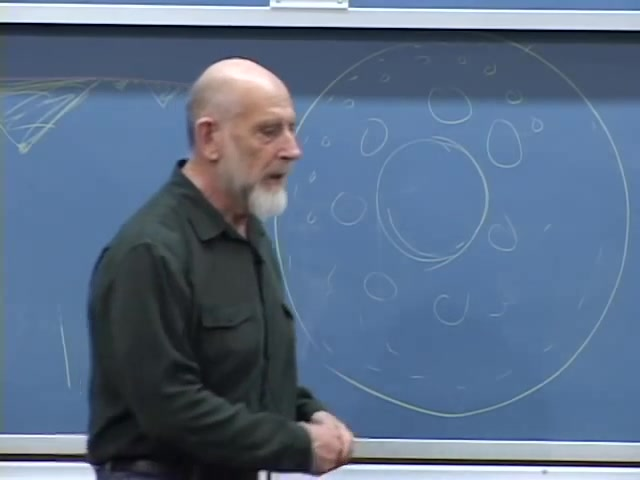
\includegraphics[width=0.76\textwidth]{lecture_09_figure_15.png}
\caption{円形の境界近くで指数関数的に増殖するエッシャーの図形に対応する黒板の代用図。}
\lectureframe{01:37:54}
\end{figure}

エッシャーが有限の時間、インク、忍耐しか持たないと想像しよう。縁の近くで彼はやがて描くのをやめ、おそらくいくつかの図形を未完成のまま残す。図形の数は双曲半径とともに指数関数的に増大するため、有限の外側の層は、描かれたすべての図形の一定の割合を含む。カットオフをどれほど外側へ動かしても、およそ半分が最終層に存在しうる。

次に天使と悪魔の比を問う。理想的な無限の模様では、対称性は一対一の等しさを示唆する。しかし任意の有限の数え上げでは、わずかに異なる境界が一方の型の図形をはるかに多く含みうる。数の大半は境界の近くにあるため、その境界の小さな変形が答えにオーダー1の変化を生む。

\begin{figure}[htbp]
\centering
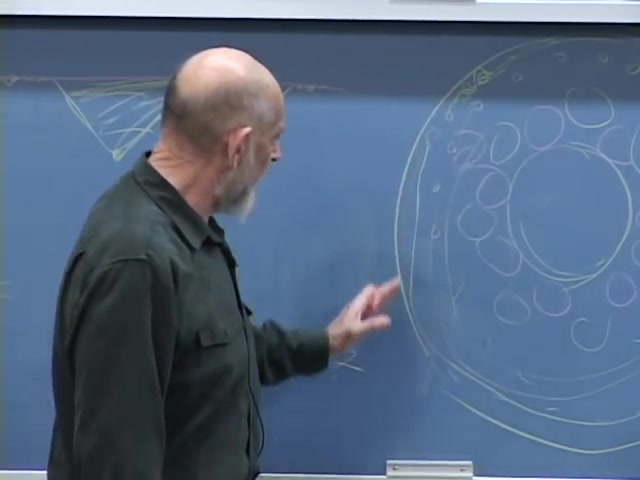
\includegraphics[width=0.76\textwidth]{lecture_09_figure_16.png}
\caption{指数関数的に増大する模様では、カットオフ境界が数の集計を支配する。}
\lectureframe{01:43:06}
\end{figure}

同じ曖昧さが永遠のインフレーションにも現れる。ある時間カットオフより下の青とピンクの泡宇宙を数え、次にカットオフをより後に押しやる。どちらの数も発散し、その比は\emph{時間}が何を意味するか、またカットオフ面がどのように描かれるかに敏感に依存しうる。確率測度とは、無限の母集団を正則化し、相対確率を抽出する処方である。異なるもっともらしい処方が一致しないことが測度問題である。

\begin{classroomqa}
\audiencequestion{このカットオフ問題と繰り込みの間に関係はありますか。\lecturetimestamp{01:45:43}}
\lecturerresponse{類推はある。量子場の理論では、格子または紫外カットオフを導入し、それを細かくし、正則化の縁の詳細に敏感でない量を求める。宇宙論者たちは永遠のインフレーションから同様に頑健な抽出を望んでいるが、ここで論じられる枠組みでは、それに匹敵する決定的な処方はまだ利用可能ではない。}
\end{classroomqa}

この類推を過大に評価すべきではない。繰り込みが成功するのは、制御された流れが正則化に依存しない観測量を特定する場合である。測度問題とはまさに、対応する不変な問いと極限手続きが不明瞭なままであるということである。われわれは間違った問いをしているのかもしれないと言うことは、正しい問いが提示されるまでは解決ではない。

\begin{classroomqa}
\audiencequestion{このバブル描像は、我々の初期宇宙におけるインフレーションと同じ現象なのか？\lecturetimestamp{01:48:19}}
\lecturerresponse{密接に関係している。永遠のインフレーションでは、親背景はインフレーションを続けながら、局所的なバブル内部は独自の宇宙論的進化を遂げる。我々の観測可能な宇宙は、そのような領域の一つの中に位置している可能性がある。}
\end{classroomqa}

\section{バブル衝突は観測できるか？}

二つのバブルは出会ったときに単に真空エネルギーを足し合わせるのではない。ドメインウォールが異なる真空状態を持つ領域を隔てており、その壁の幾何学がどちら側で何を観測できるかを決める。衝突の位置が我々の過去光円錐に対してどこにあるかに応じて、その痕跡は隠されることもあれば可視となることもある。

\begin{classroomqa}
\audiencequestion{二つの真空バブルが衝突すると何が起こるのか？\lecturetimestamp{01:52:07}}
\lecturerresponse{衝突はドメインウォールの幾何学を生み出し、その振る舞いは二つの真空と壁の張力に依存する。好都合な因果的条件の下では、その擾乱は我々の観測可能な領域に入り込み、異方的な痕跡を残しうる。}
\end{classroomqa}

この講義では、宇宙マイクロ波背景放射における低温領域を可能な候補として論じ、円形の特徴の周囲の偏光を判別要因として指摘する。これは意図的に、検出ではなく可能性として提示されている。説得力のある衝突の痕跡は革命的であろう。なぜなら、隣接するバブル領域の直接的な証拠を与え、測度問題を実験的に緊急のものとするからである。

\begin{figure}[htbp]
\centering
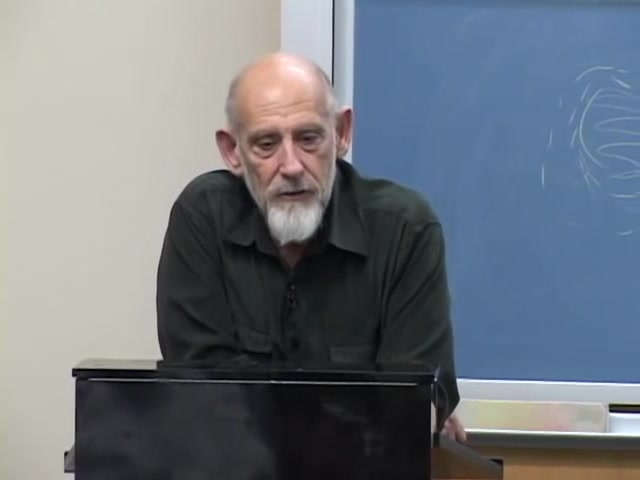
\includegraphics[width=0.70\textwidth]{lecture_09_figure_17.png}
\caption{バブル衝突の議論における円形の空の特徴とその可能な偏光パターン。}
\lectureframe{01:50:22}
\end{figure}

\editorialnote{低温スポットの議論は、講義当時の観測状況と提案を記録したものである。温度異常それ自体はバブル衝突の証拠ではなく、詳細で相関した痕跡が必要とされる。}

\begin{classroomqa}
\audiencequestion{バブルは四次元なのか、またその内部はどのような空間曲率を持つのか？\lecturetimestamp{01:53:37}}
\lecturerresponse{それらは時空領域であり、外部の時間の中で進化する三次元の石鹸膜ではない。その内部は典型的には負の空間曲率を持つ開いたFRW宇宙である。衝突はその幾何学を摂動するが、負の曲率を単純に正の曲率に変えるわけではない。}
\end{classroomqa}

\section{弦理論が確立することと確立しないこと}

最後の議論は、弦理論が正しい確率を割り当てるよう促すところから始まる。サスキンドは、その命題が曖昧すぎるとして数値を拒否する。代わりに彼は二つの主張を区別する。

第一に、量子力学と重力を組み合わせた高度に制約された数学的構造がある。それは精密な結果と深い数学的同一性を生み出し、その内部整合性は広範な精査に耐えてきた。講義の非公式な用語では、これは大文字の\(S\)を伴う\emph{String Theory}である。最も鋭く理解されている版は、超対称性に大きく依存している。

第二に、観測される世界は到達可能なエネルギーでは超対称ではない。厳密な超対称的構成を我々の非超対称的な宇宙に結びつけるには、超対称性の破れと、同じ精度では制御されないより大きな枠組みが必要である。講義の用語では、その望まれる拡張は小文字の\(s\)を伴う\emph{string theory}である。

\begin{classroomqa}
\audiencequestion{弦理論が自然の正しい理論である確率を割り当てることはできるか？\lecturetimestamp{01:54:18}}
\lecturerresponse{どの主張を意味するのかを特定せずに責任を持って行うことはできない。厳密な数学的構造は存在し、量子重力を含んでいるが、厳密に制御された超対称的模型は文字通り我々の観測する世界ではない。より大きな拡張が我々の世界を含むかどうかは、物理学者が情報に基づく先入観を持ちうる事柄であり、明確に定義された数値的確率ではない。}
\end{classroomqa}

完全な数学的機構が利用可能になる前の力学との類推である。\(F=ma\)と逆二乗の力を知っていても、高度に対称な円軌道しか解けないかもしれない。解ける部門は本物であろうが、理論全体ではない。同様に、厳密な超対称的弦構成は、より大きな構造の特別で異常に扱いやすい領域かもしれない。

\begin{figure}[htbp]
\centering
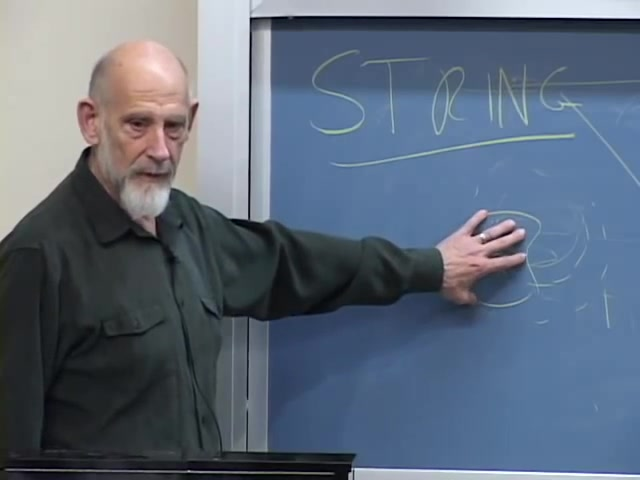
\includegraphics[width=0.60\textwidth]{lecture_09_figure_18.png}
\caption{講義の入れ子描像：推測的により大きな枠組みの中にある、厳密に制御された超対称的弦構成。}
\lectureframe{01:57:34}
\end{figure}

\begin{classroomqa}
\audiencequestion{なぜ厳密理論において単純に超対称性を破らないのか。\lecturetimestamp{01:57:02}}
\lecturerresponse{多くの近似的構成が超対称性の破れを研究しているが、完全に制御された非超対称的な骨格こそがまさに欠けているものである。標準的な近似を行った後に計算することはできるが、それらの近似が近づいていく厳密な対象を常に知っているわけではない。}
\end{classroomqa}

\begin{classroomqa}
\audiencequestion{厳密な超対称理論は、我々の世界を含むより大きな、より対称性の低い拡張を排除するのか。\lecturetimestamp{02:00:33}}
\lecturerresponse{否。それは観測される世界が厳密な超対称的セクターのみによって記述されないことを確立する。このセクターが現実的な物理を含むより大きな理論と結びついていることを証明も反証もしない。}
\end{classroomqa}

\begin{classroomqa}
\audiencequestion{弦の構成は、素粒子物理学の対称性の破れに類似した対称性の破れを含むのか。\lecturetimestamp{02:01:21}}
\lecturerresponse{超対称性の破れに関する広範な研究があり、超対称的な数学については多くが知られている。未解決の点は、現実的な破れを制御された近似のみならず完全な理論と組み合わせる、精密な非摂動的定式化である。}
\end{classroomqa}

\begin{classroomqa}
\audiencequestion{特殊相対性理論は弦理論において要請されるのか、それとも予言として現れるのか。\lecturetimestamp{02:03:02}}
\lecturerresponse{基礎となる規則はローレンツ不変である。たとえ物質で満たされた特定の背景が好ましい静止系を選び出しうるとしても。重力はさらに避けがたい。弦のスペクトルは、重力子の相互作用を持つ質量ゼロのスピン2の励起を含む。}
\end{classroomqa}

\begin{classroomqa}
\audiencequestion{弦理論は一般相対性理論および背景独立性と整合するのか。\lecturetimestamp{02:04:11}}
\lecturerresponse{その低エネルギー重力動力学は一般相対性理論と整合し、局所的な背景は動的に変化しうる。微妙な点は漸近的境界条件にある。それらは問題そのものを指定するものであり、一般にその時空内の局所的操作によって変えることはできない。}
\end{classroomqa}

講義は、堅牢な数学的核と未完成の物理的外挿との間のその区別で閉じられる。それは核が無用であるという判定でもなく、外挿が確立されたという主張でもない。厳密な知識がどこで終わるかを述べたものである。
